\chapter{Технологический раздел}
В данном разделе подготовлены данные для обучения и тестирования модели рекомендаций, а также реализована рекомендательная система в виде программы.

\section{Подготовка данных}
Для того, чтобы применить рекомендательную модель, необходимо получить её параметры.
Процесс их получения называется обучением модели~\cite{aggarwal}.
Чтобы обучить модель требуется подготовить набор данных.
Согласно техническому заданию, эти данные должны содержать рецепты и реальные данные об их оценках какими-либо пользователями.
Причём рецепты в подготовленном наборе данных должны включать в себя все свойства, представленные на диаграмме~\ref{fig:er}.
В ходе выполнения работы найден источник данных, удовлетворяющих сформулированным условиям~\cite{recipe_dataset}.
Исходные данные представлены на английском языке, следовательно, необходимо выполнить их перевод.
Был проведён выбор $1000$ рецептов, которые затем переведены на русский язык для удовлетворения цели работы.
Результат подготовки данных сохранён в таблицу, фрагмент которой представлен на рисунке~\ref{fig:dataset}.
\begin{figure}[htbp]
	\centering
	\imgfig{img/dataset}
	\caption{
	    Фрагмент подготовленного набора данных для обучения и тестирования рекомендательной модели
	}
	\label{fig:dataset}
\end{figure}

\section{Выбор средств разработки}
Сначала проведён выбор операционной системы.
Существующие аналоги предназначены для использования на мобильных устройствах~\cite{app_tasty}~\cite{app_easyrecipes}~\cite{app_foodru}.
Поэтому была выбрана операционная система Android как самая популярная для таких устройств ~\cite{ghazawneh2013dual}.
Для реализации приложения под Android самыми современными средствами является следующее~\cite{android_developers}:
\begin{itemize}
	\item язык программирования Kotlin;
	\item средство разработки интерфейсов Jetpack Compose;
	\item среда разработки Android Studio.
\end{itemize}
Для внедрения в приложение шаблона проектирования MVI использована библиотека <<Decompose>>~\cite{arkivanov}.
Она предоставляет полный набор возможностей не только для связи интерфейса с прецедентами, но и для навигации между отображаемыми окнами приложения.
Чтобы обеспечить инъекцию зависимостей на этапе компиляции, выбрана библиотека <<Dagger>>~\cite{dagger}.
Она позволяет избежать ошибок, связанных и инициализацией объектов, во время выполнения программы.
Для реализации базы данных требуется средство как локального, так и удалённого хранения данных.
Локальное хранение в Android обеспечивается базой данных <<SQLite>>~\cite{room}.
Она является реляционной, не имеет ролевой модели и предоставляет все необходимые типы данных.
Библиотека Room является самой популярной для доступа к рассматриваемой базе данных, поэтому именно она была выбрана для реализации локального хранения данных~\cite{room}.
Удалённое хранение сущностей обеспечивается документальной базой данных <<Firebase>>~\cite{firebase}.
Она предоставляет не только хранение данных о пользователях, но и средство их авторизации в системе.

В результате выбранные технологии предоставляют все необходимые возможности для реализации рекомендательной системы в виде мобильного приложения и рекомендуются к использованию компанией, развивающей операционную систему Android~\cite{android_developers}.

\section{Реализация рекомендательной системы}
Реализованное приложение содержит следующие слои:
\begin{itemize}
	\item <<database>> -- база данных;
	\item <<data>> -- слой обработки данных;
	\item <<domain>> -- слой, содержащий объявления основных сущностей, интерфейсов и прецедентов;
	\item <<presentation>> -- слой с реализацией интерфейса и взаимодействия с пользователем.
\end{itemize}

Слой <<presentation>> разделён на следующие компоненты, каждый из которых представляет собой графический интерфейс, реализующий набор возможностей:
\begin{itemize}
	\item <<profile>> -- профиль пользователя;
	\item <<authorization>> -- авторизация пользователя;
	\item <<details>> --  отображение информации о рецепте и интерфейса работы с ним;
	\item <<favourites>> -- отображение избранных рецептов;
	\item <<initialization>> -- инициализация базы данных при первом запуске приложения;
	\item <<recommend>> -- запрос и получение рекомендаций;
	\item <<scores>> -- отображение оценок и интерфейс работы с ними;
	\item <<search>> -- поиск рецептов.
\end{itemize}
Есть ещё один компонент приложения -- <<navigation>>, который реализует переключение между вышеперечисленными графическими интерфейсами.
Реализация всего приложения оформлена в виде приложения <<Б>>.

\section{Реализация получения векторов рецептов}
Для того, чтобы применить методы контентной фильтрации, выбранные рецепты необходимо представить в виде векторов вещественных чисел.
Это делается с помощью метода, описанного на этапе анализа.
В приложении <<В>>, в листингах~\ref{lst:rvec_1}--\ref{lst:rvec_4}, представлена реализация получения векторов признаков на языке <<Python>>.
После извлечения признаков проведена их нормализация по формуле~\ref{eq:std_norm} с целью повысить качество алгоритма предсказания оценок.
Таким образом, получены данные, необходимые для формирования рекомендаций.
При первом запуске приложения происходит загрузка векторов рецептов из удалённой базы данных, после чего рекомендательная система готова к работе.

\section{Примеры работы программы}
На рисунках~\ref{fig:search}--\ref{fig:scores} приведены фотографии интерфейса реализованной программы в процессе её тестирования.
Рисунок~\ref{fig:recommend} отображает пример работы рекомендательной системы на одном тестовом случае.
Таким образом, продемонстрированы результаты тестирования разработанной рекомендательной системы.
\begin{figure}[htbp]
	\centering
	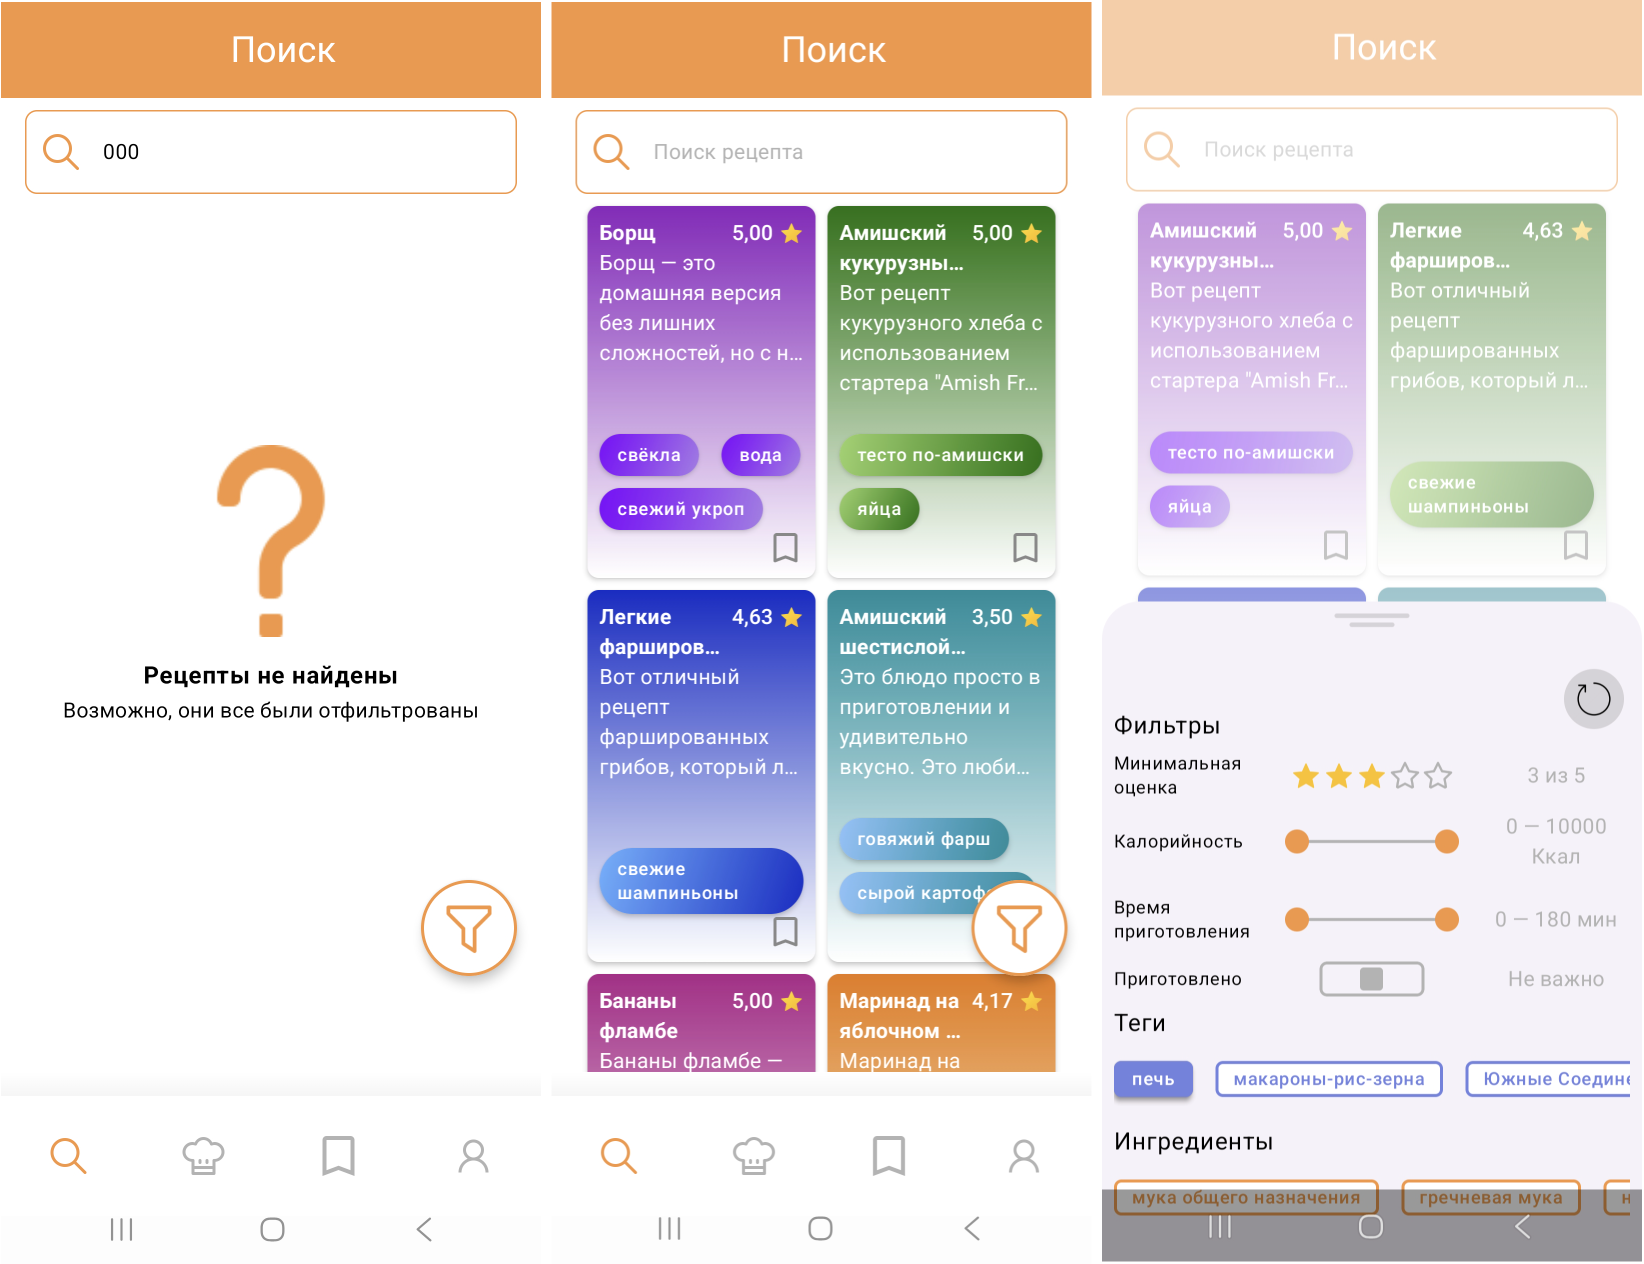
\includegraphics[height=0.45\textheight]{img/search.png}
	\caption{
	    Разработанное приложение, интерфейс поиска
	}
	\label{fig:search}
\end{figure}
На рисунке~\ref{fig:search} представлен интерфейс поиска.
Левое изображение демонстрирует пустой результат поиска, а центральное -- результат успешного поиска.
На правом изображении показан интерфейс для задания параметров фильтрации рецептов.
Далее на рисунке~\ref{fig:details} представлен раздел приложения с информацией о рецепте.
Он отображает следующее:
\begin{itemize}
	\item название;
	\item описание;
	\item прокручиваемый список ингредиентов;
	\item шаги приготовления блюда;
	\item информация о калорийности;
	\item кнопка, помечающая рецепт как приготовленный;
	\item оценка рецепта;
	\item кнопка удаления оценки.
\end{itemize}
Если пользователь авторизован, то он может присвоить рецепту оценку, нажав на соответствующий её элемент.
Когда оценка сохранена, она отображается на экране.
Если пользователь не авторизован в системе, то кнопка сохранения оценки не активна.
\begin{figure}[htbp]
	\centering
	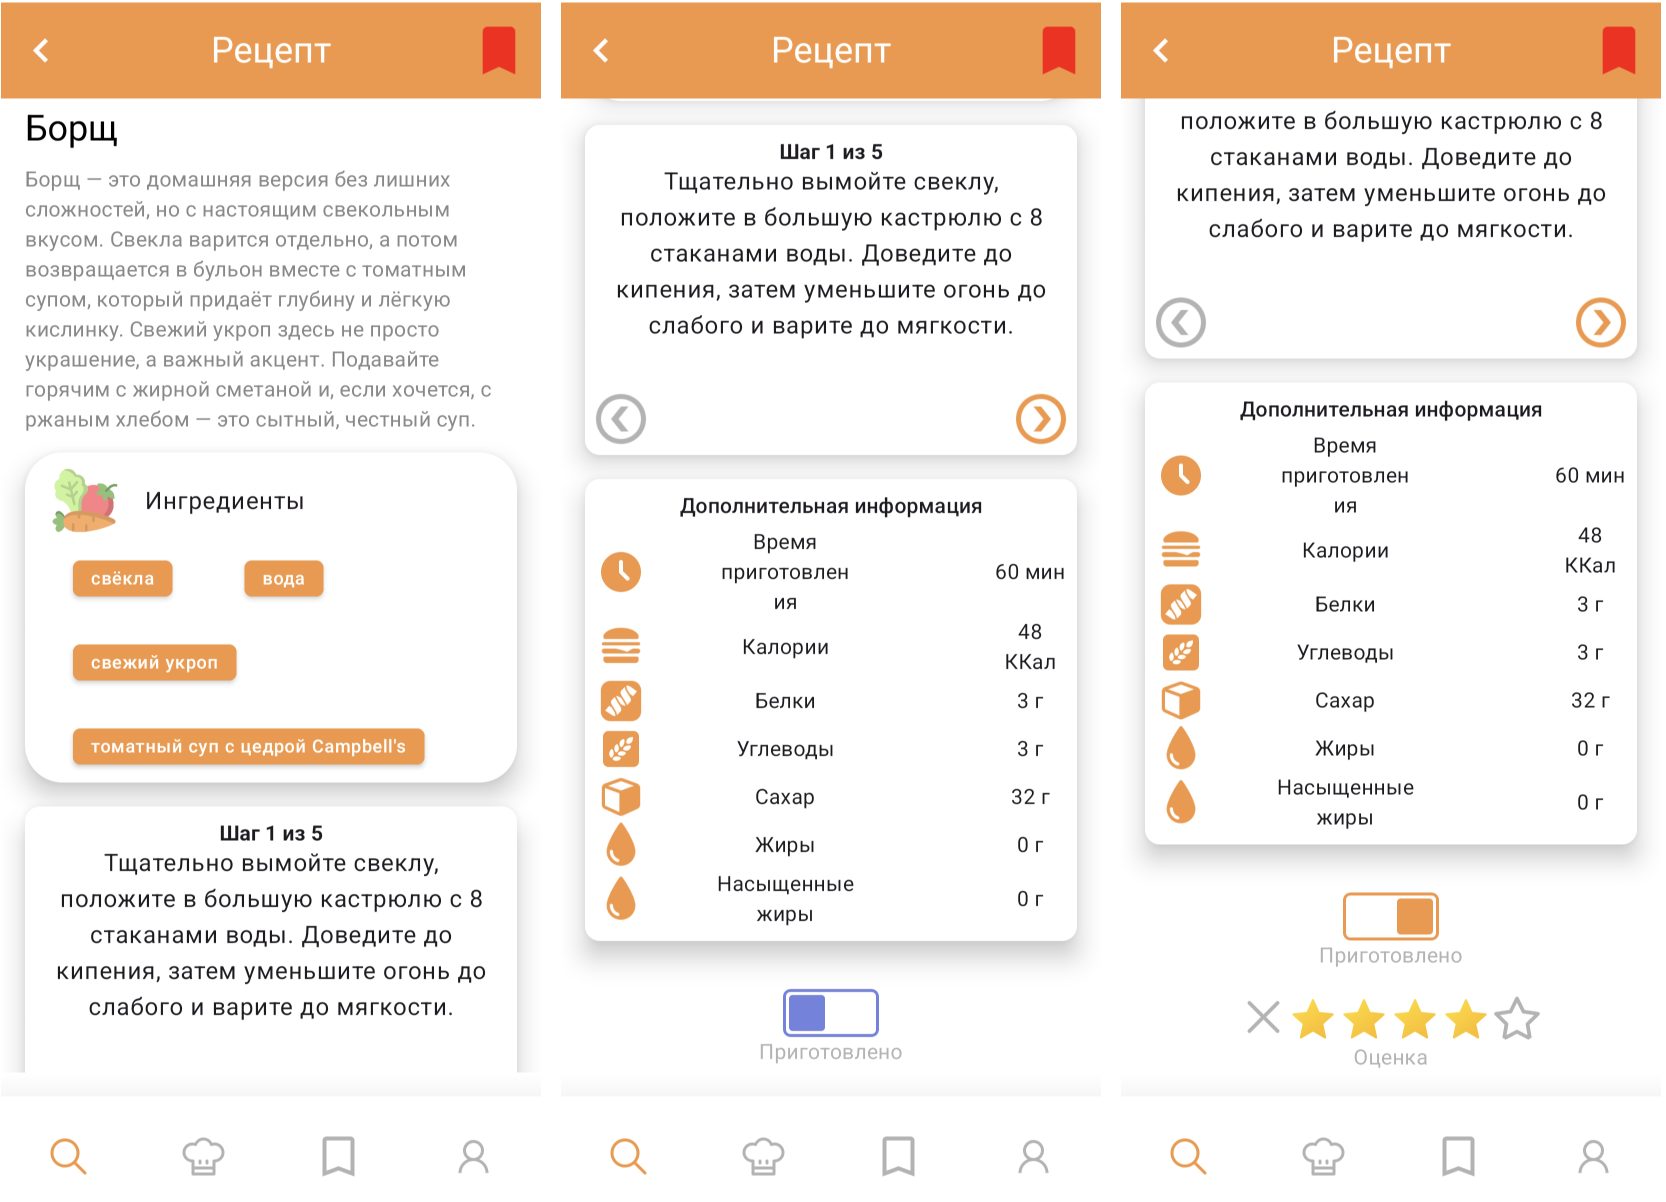
\includegraphics[height=0.45\textheight]{img/details.png}
	\caption{
	    Разработанное приложение, раздел информации о рецепте
	}
	\label{fig:details}
\end{figure}
На рисунке~\ref{fig:favourites} представлен интерфейс для работы со списком избранных рецептов.
Слева изображён раздел избранного при отсутствии авторизованного пользователя.
По центру показан интерфейс этого раздела при отсутствии каких либо рецептов в избранном: отображаются кнопки, открывающие раздел поиска и рекомендаций.
На правом изображении видно, как выглядит интерфейс избранного при наличии в нём рецептов.
Рисунок~\ref{fig:authorize} демонстрирует раздел авторизации: на левом изображении представлено начальное состояние, на центральном -- интерфейс регистрации нового пользователя, а на правом -- интерфейс входа.
На рисунке~\ref{fig:scores} представлен раздел оценок.
Слева изображён список всех оценок, а справа -- оценок приготовленных рецептов.
\begin{figure}[htbp]
	\centering
	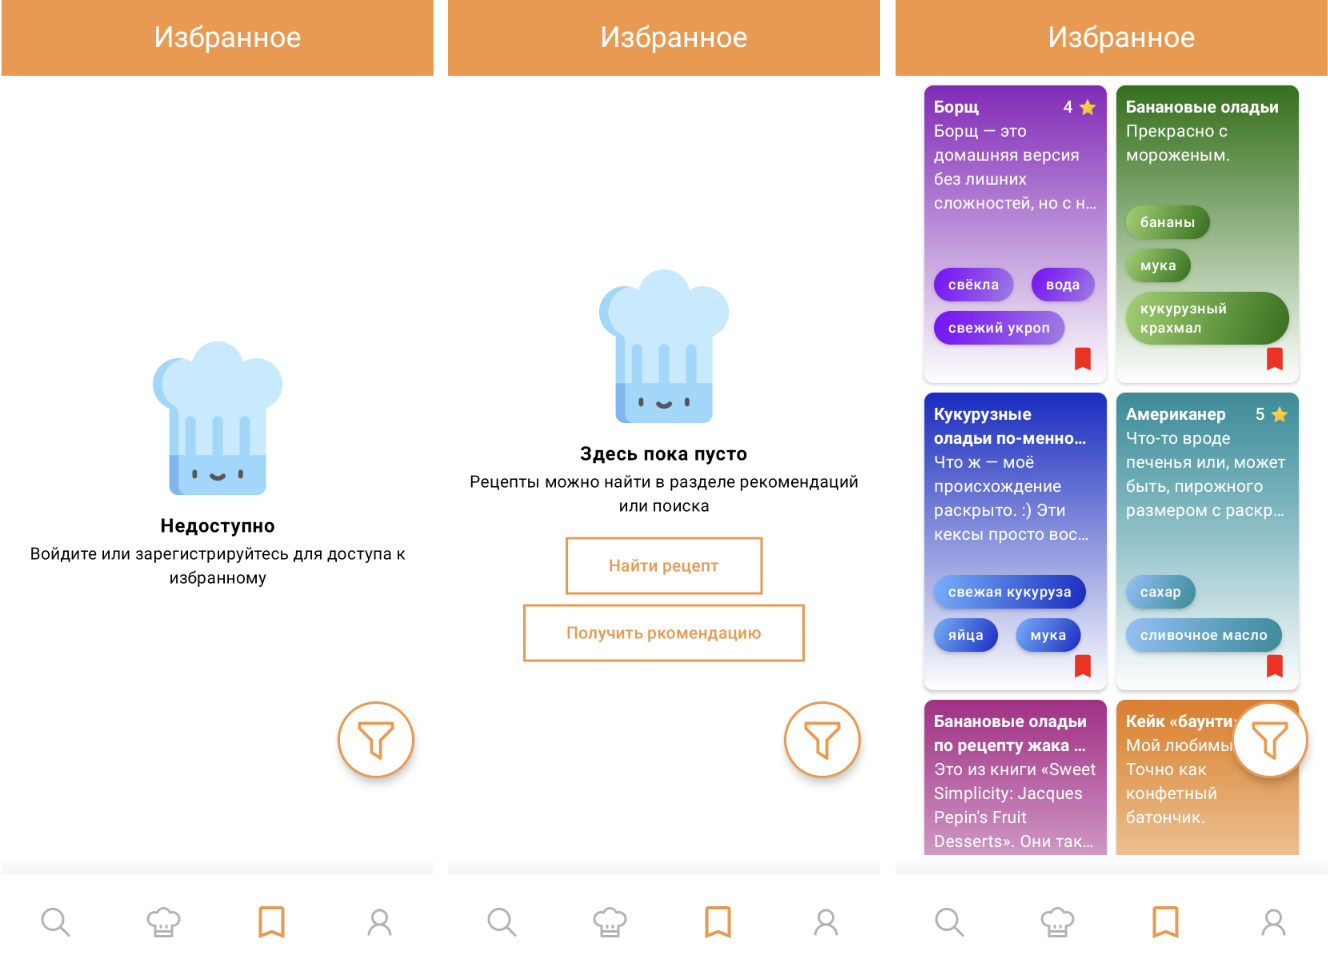
\includegraphics[height=0.45\textheight]{img/favourites.png}
	\caption{
	    Разработанное приложение, раздел избранного
	}
	\label{fig:favourites}
\end{figure}
\begin{figure}[htbp]
	\centering
	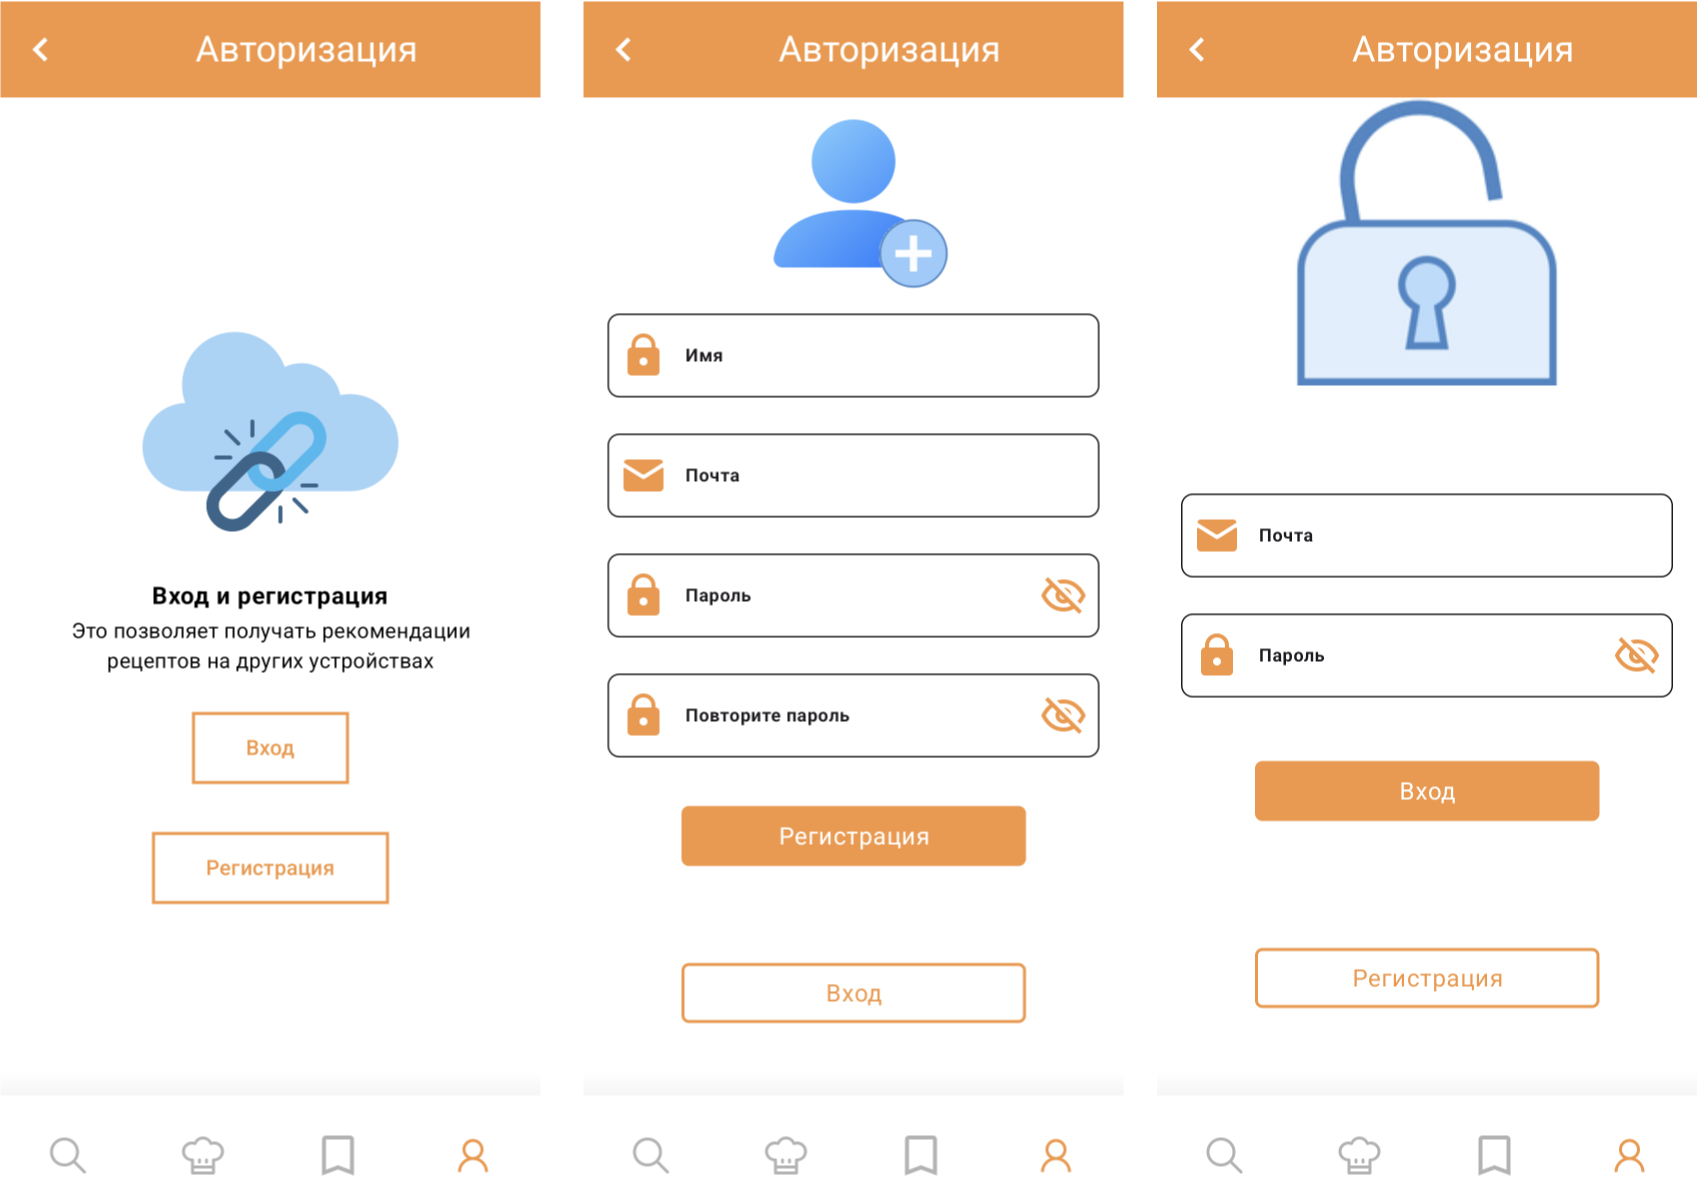
\includegraphics[height=0.45\textheight]{img/authorize.png}
	\caption{
	    Разработанное приложение, раздел авторизации
	    }
	\label{fig:authorize}
\end{figure}
\begin{figure}[htbp]
	\centering
	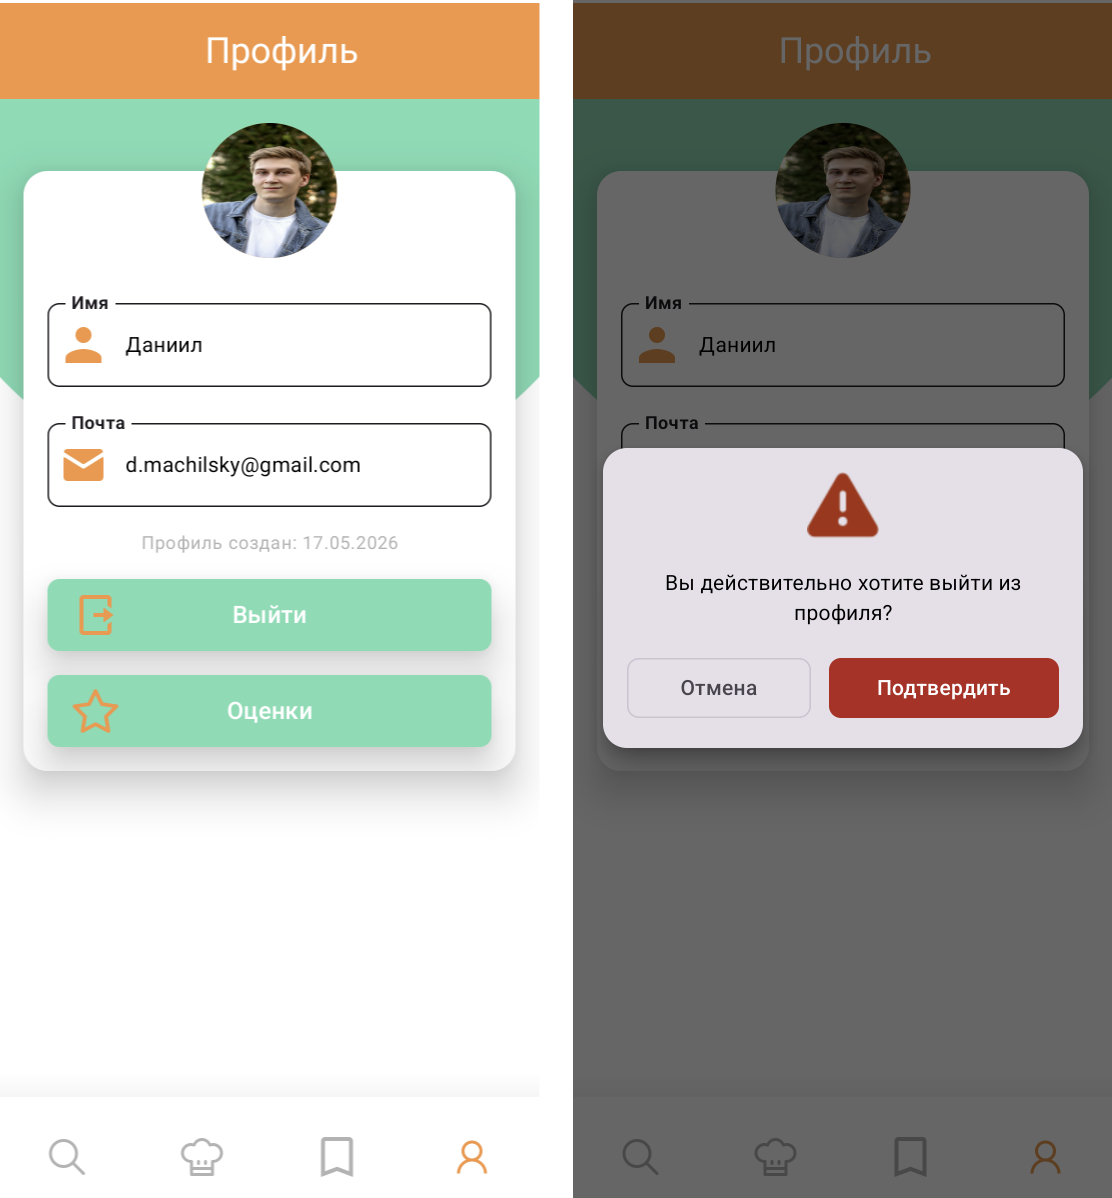
\includegraphics[height=0.45\textheight]{img/profile.png}
	\caption{
	    Разработанное приложение, раздел профиля
	}
	\label{fig:profile}
\end{figure}
\begin{figure}[htbp]
	\centering
	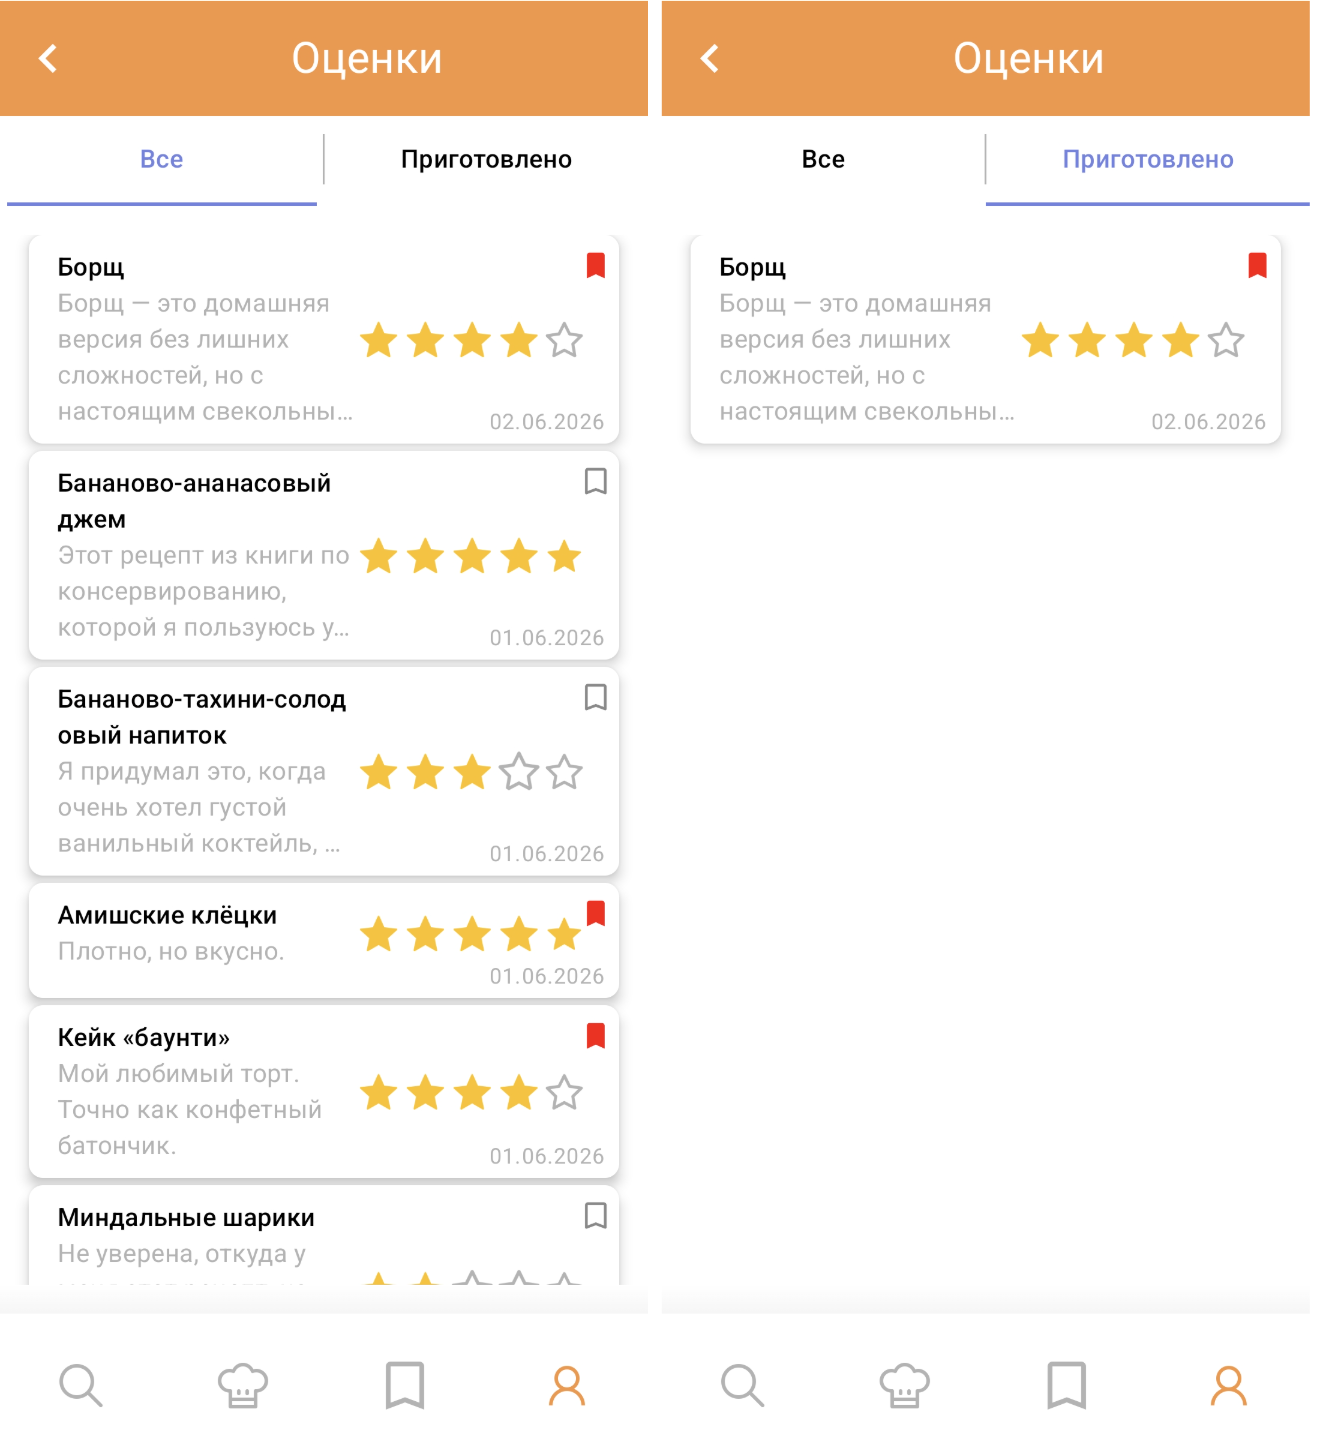
\includegraphics[height=0.45\textheight]{img/scores.png}
	\caption{
	    Разработанное приложение, раздел оценок
	}
	\label{fig:scores}
\end{figure}
\begin{figure}[htbp]
	\centering
	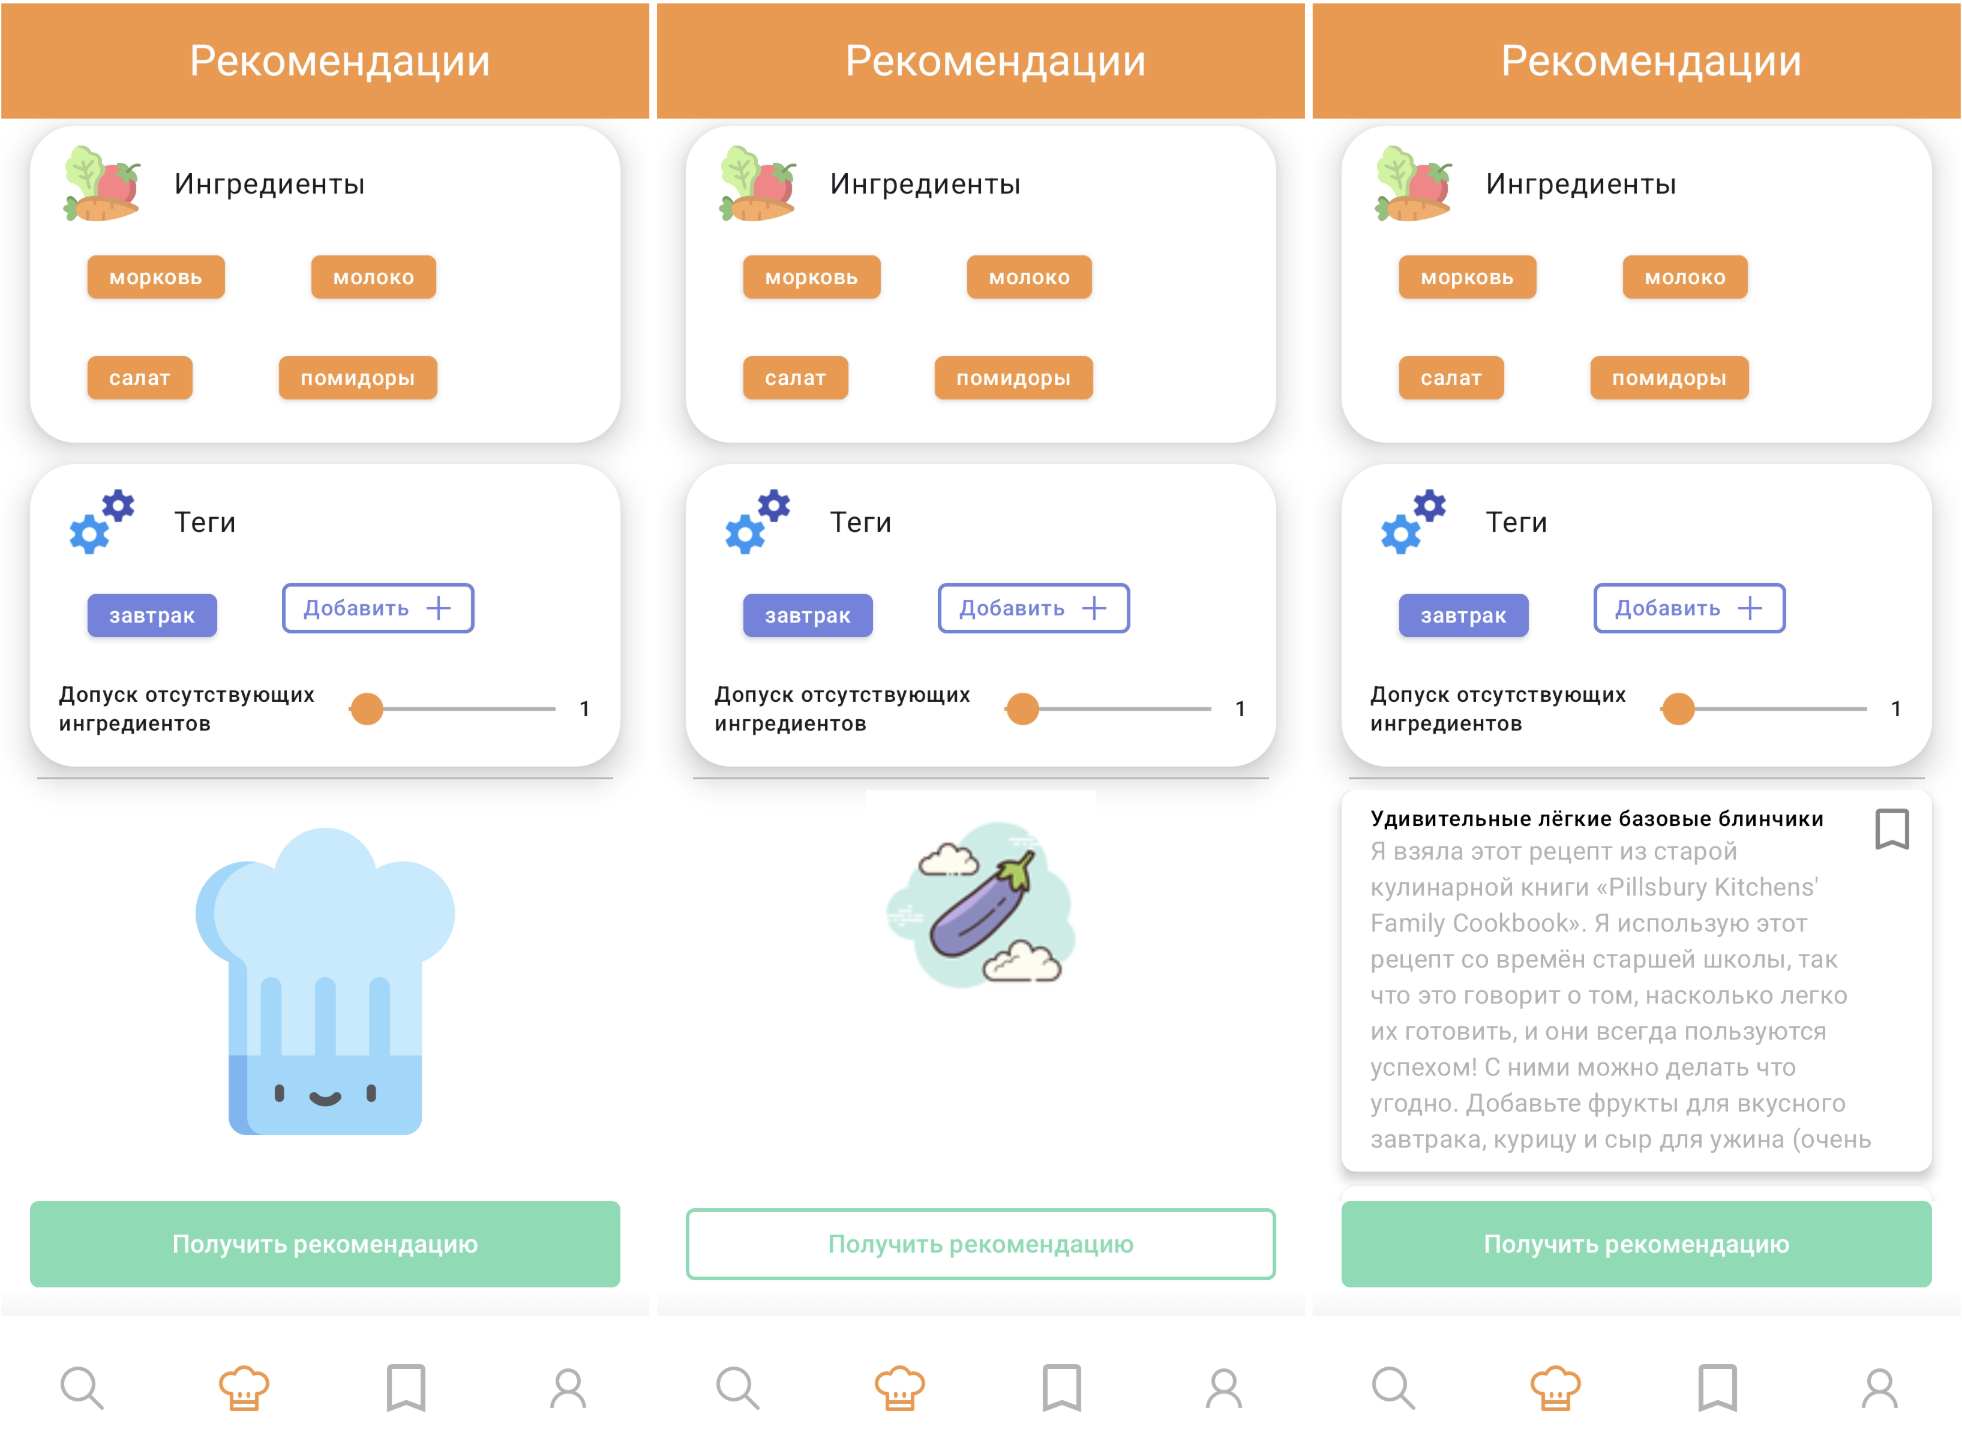
\includegraphics[height=0.45\textheight]{img/recommend.png}
	\caption{
	    Разработанное приложение, раздел рекомендаций
	}
	\label{fig:recommend}
\end{figure}
Результат тестирования функции получения рекомендаций представлен на рисунке~\ref{fig:recommend}.
Введён список ингредиентов и дополнительные фильтры в виде тегов и максимального количества отсутствующих ингредиентов.
Результат ввода приведён на левом изображении.
Центральное изображние демонстрирует состояние интерфейса при загрузке рекомендаций.
На правом показан список рекомендованных рецептов.
Таким образом, в результат тестирования успешно получена рекомендация.

\section*{Вывод из технологического раздела}
В результате данного раздела выбраны технологии реализации рекомендательной системы, подготовлен набор данных для её тестирования и приведена реализация получения векторов рецептов.
Также представлены результаты тестирования программы в виде изображений её интерфейса.
Таким образом, получено программное обеспечение для исследования его характеристик.
Следовательно, цель раздела достигнута.

